\section*{Results} 
\subsection*{Numerical Stroop Accuracy} 
\begin{figure}[t]
    \centering 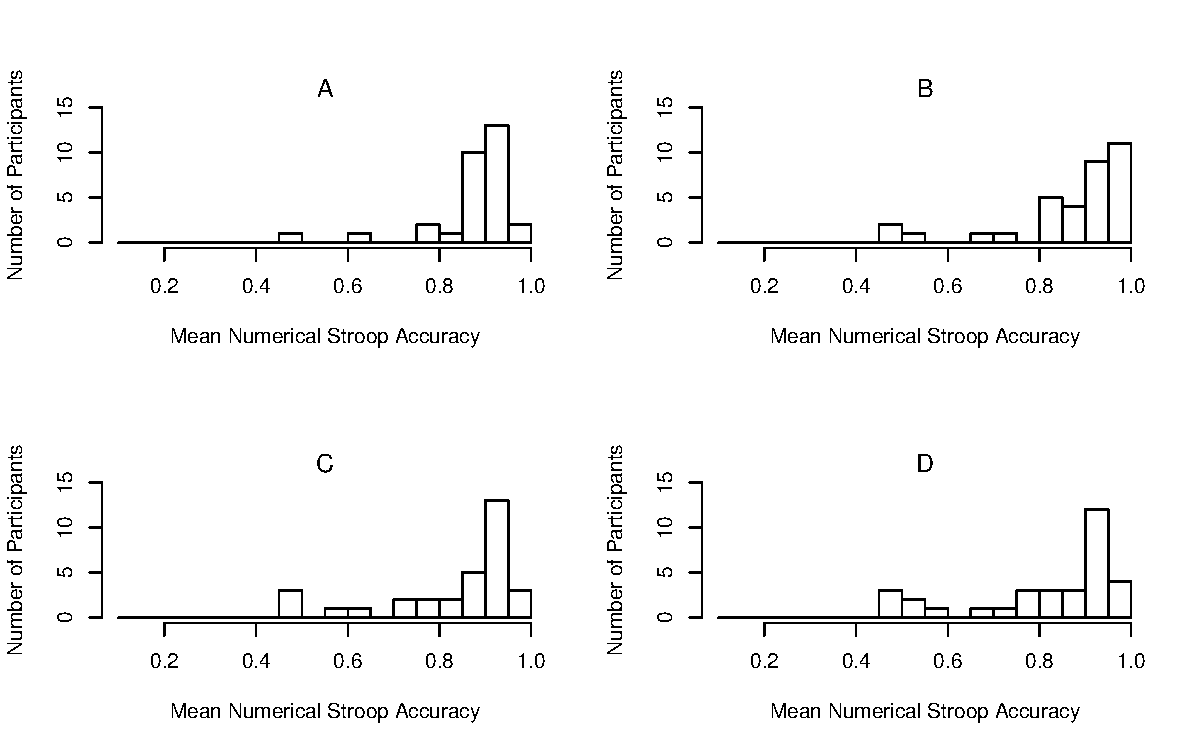
\includegraphics[width=1.0\textwidth]{../figures/fig_exc_dual.pdf}
    \caption{
      Histograms showing distribution of mean Numerical Stroop accuracy
      seperately for each condition. 
      \textbf{A:} Condition 1.
      \textbf{B:} Condition 2.
      \textbf{C:} Condition 3.
      \textbf{D:} Condition 4.
    }
    \label{fig:exc_dual}
\end{figure}

Figure \ref{fig:exc_dual} shows histograms characterizing mean dual-task
performance seperately for each condition. Overall, mean accuracy on the
dual-task was very good, with mean proportion correct at $0.88$ in Condition 1,
$0.87$ in Condition 2, $0.84$ in Condition 3, and $0.82$ in Condition 4.

\subsection*{Classification Accuracy} 
\begin{figure}[t]
  \centering 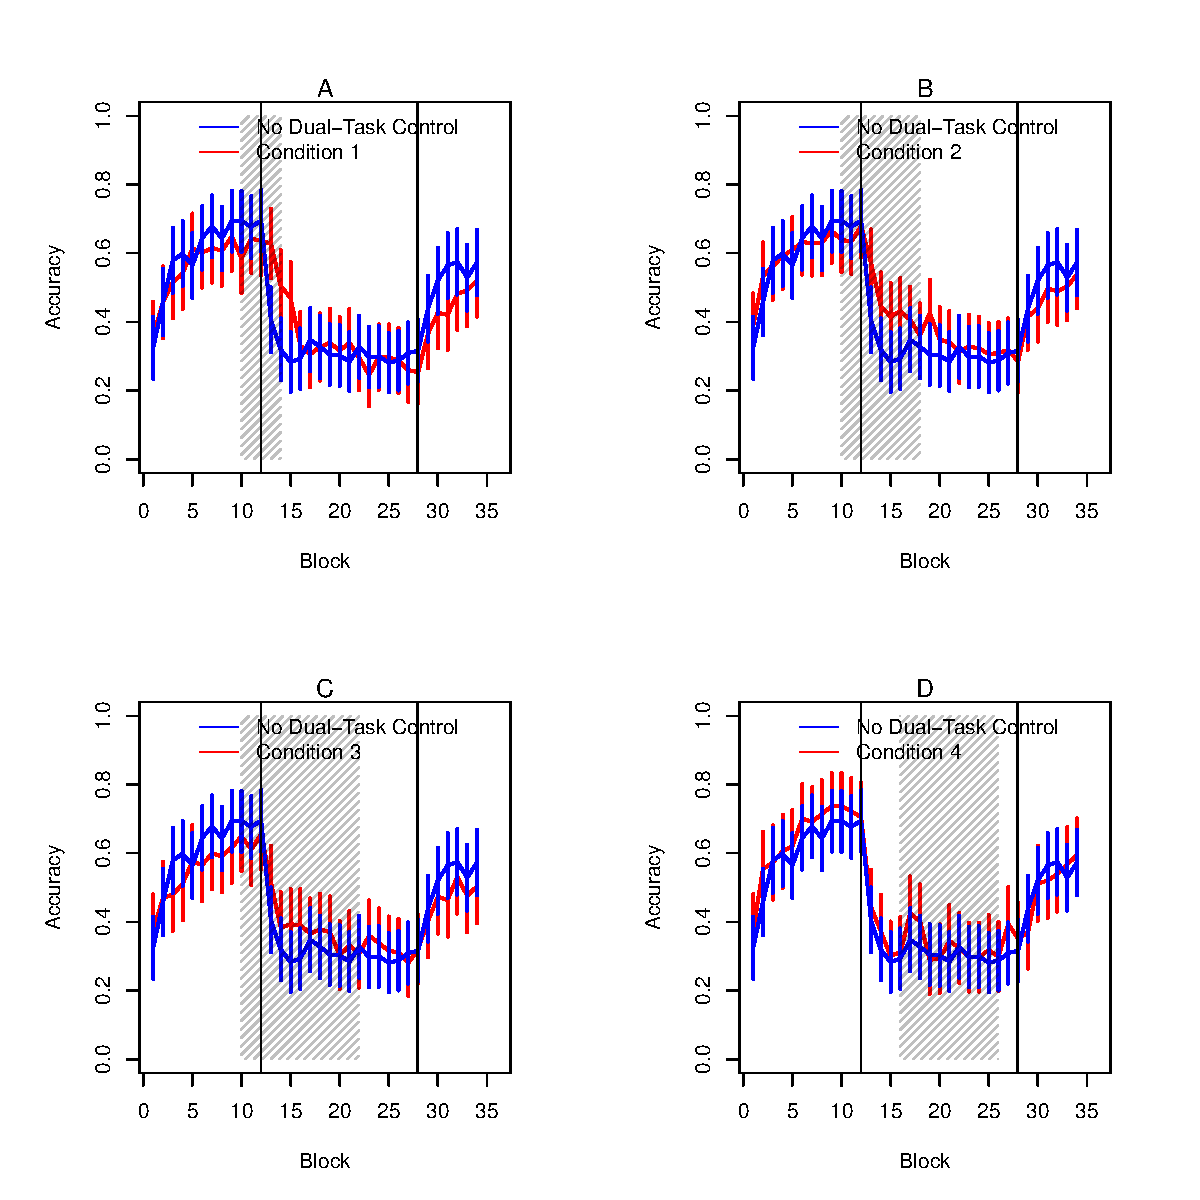
\includegraphics[width=1.0\textwidth]{../figures/fig_learning_curves.pdf}
  \caption{
    Mean accuracy per 25 trial block. The blue line in each panel is Condition
    5 (no dual-task control). The hatch marks indicate dual-task trials. The key
    features are (1) dual-task slows the change in classification strategy (seen
    in this plot as ``accuracy'' decline), and (2) the dual-task conditions show
    less savings than the no dual-task control. There is no obvious 
    dose-dependent effect of the dual task, nor is there an obvious difference
    between dual-task conditions.
    \textbf{A:} Condition 1 (dual-task applied on trial 251 through trial 350).
    \textbf{B:} Condition 2 (dual-task applied on trial 251 through trial 450). 
    \textbf{C:} Condition 3 (dual-task applied on trial 251 through trial 550). 
    \textbf{D:} Condition 4 (dual-task applied on trial 351 through trial 650). 
    Error bars are SEM.
  }
  \label{fig:learning_curves}
\end{figure}

Figure \ref{fig:learning_curves} shows the mean accuracy in each block of 25
trials across the duration of the experiment. Recall that if feedback
contingency is estimated via declarative mechanisms, then (1) dual-task trials
should slow the change in classification performance during intervention, and
(2) dual-task conditions should show reduced savings relative to the no
dual-task control. We see evidence for both features in our data.

\subsubsection*{Acquisition}
Conditions 1 -- 5 are identical for the first 250 trials (10 blocks) of
acquisition (before dual-task onset), and so we expect performance during these
blocks to be the same across conditions. This is clearly the case by visual
inspection of Figure \ref{fig:learning_curves}, and is supported by the results
of a 5 Condition $\times$ 10 Block ANOVA. The main effect of Condition was
nonsignificant [$F(4,1620) = 1.89, p = 0.11, \Omega^2 = 0.00$], and so was the
Condition $\times$ Block interaction [$F(4,1620) = 1.08, p = 0.37, \Omega^2 =
0.00$]. However, there was a significant effect of Block [$F(1,1620) = 191.00, p
< 0.001, \Omega^2 = 0.10$], reflecting improvement across the acquisition phase.

\subsubsection*{Intervention}
If the estimation of feedback contingency depends on declarative mechanisms,
then we expect change in performance during intervention to be slowed during the
simultaneous performance of the dual task. This is clearly seen in Figure
\ref{fig:learning_curves}, and is supported by the results of a 5 condition
$\times$ 14 block ANOVA. A significant effect of Condition [$F(4,2598) = 9.74, p
= 0.00, \Omega^2 = 0.01$] reflected an overall difference in intervention
performance in dual-task conditions relative to the no dual-task control. A
significant effect of Block [$F(1,2598) = 166.65, p < 0.001, \Omega^2 = 0.06$]
reflected the change in classification performance across intervention seen in
all conditions. The Condition $\times$ Block interaction was also significant
[$F(4,2598) = 14.64, p < 0.001, \Omega^2 = 0.02$], reflecting the slower change
in performance in the dual-task conditions relative to the no dual-task control.

The directional interpretation of the omnibus tests is supported by several
planned comparisons on the overall mean accuracies during the intervention
phase. First, intervention accuracy in all dual-task conditions was
significantly different from intervention accuracy in the no dual-task
control 
[condition  1 > condition  5: $t(940) = 2.78$, $p < .05, d = 0.25$;
condition  2 > condition  5: $t(1046) = 5.31, p < .01, d = 0.87$;
condition  3 > condition  5: $t(962) = 5.45, p < .01, d = 0.96$;
condition  4 > condition  5: $t(996) = 2.99$, $p < .01, d = 0.28$].
Second, the dual task slowed the accuracy drop during intervention only in
conditions in which it was first introduced during the acquisition phase
[condition  2 > condition  4: $t(1063) = 1.94, p = 0.05, d = 0.12$;
condition  3 > condition  4: $t(1037) = 2.24$, $p = 0.03, d = 0.16$],
although this difference was not observed in condition 1 (shortest dual-task
exposure)
[condition  1 > condition  4: $t(1006) = -0.23$, $p = 0.82, d = 0.00$].

\subsubsection*{Savings: Group Level}
\begin{figure}[t]
  \centering 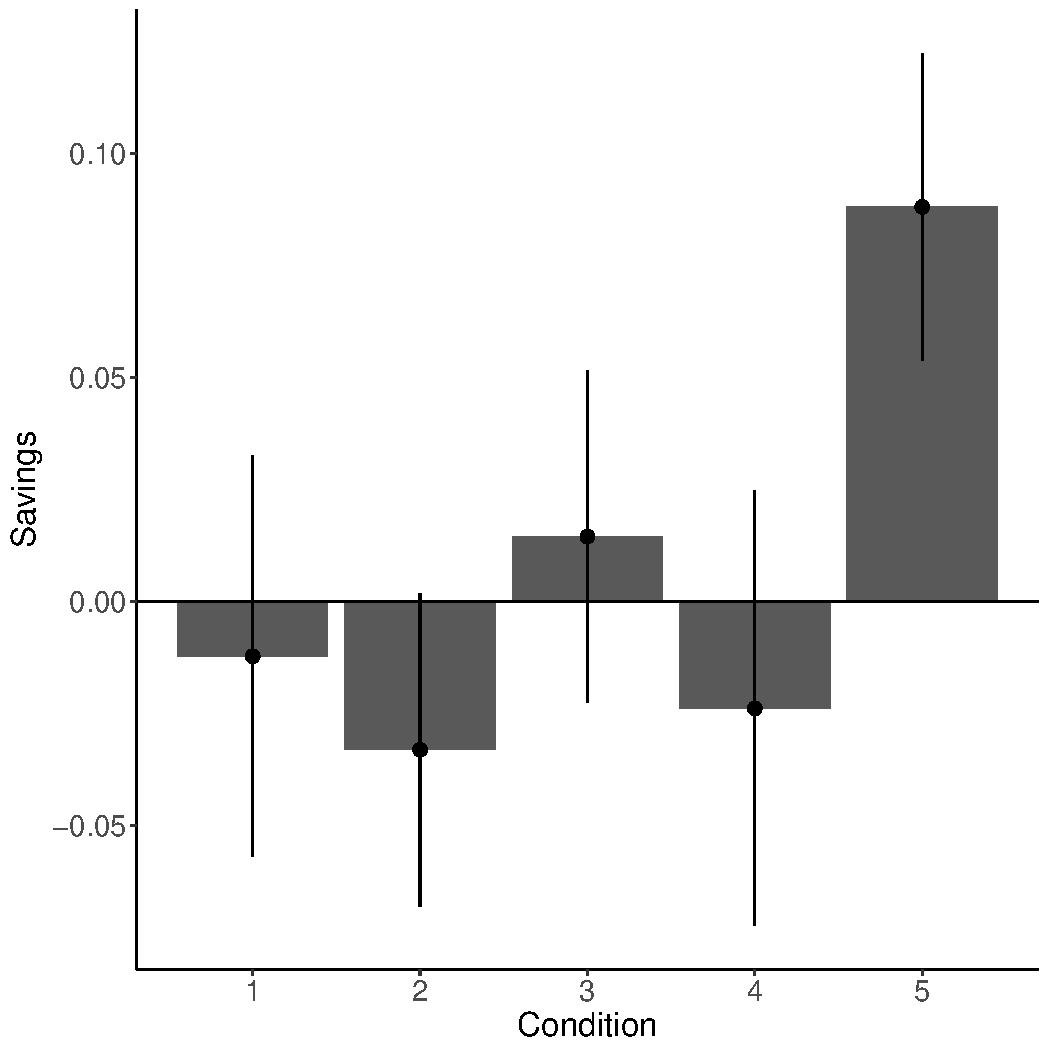
\includegraphics[width=1.0\textwidth]{../figures/fig_savings.pdf}
  \caption{ savings (mean of all 150 reacquisition trials - mean of the first
    150 acquisition trials) in all conditions of the present experiment, and also
    including data from the random feedback condition of crossley et al. (2013),
    which shows the savings observed in a no dual-task control condition with only
    300 trials of intervention. Each circle corresponds to a single participant. }
  \label{fig:savings}
\end{figure}

\begin{figure}[t]
  \centering 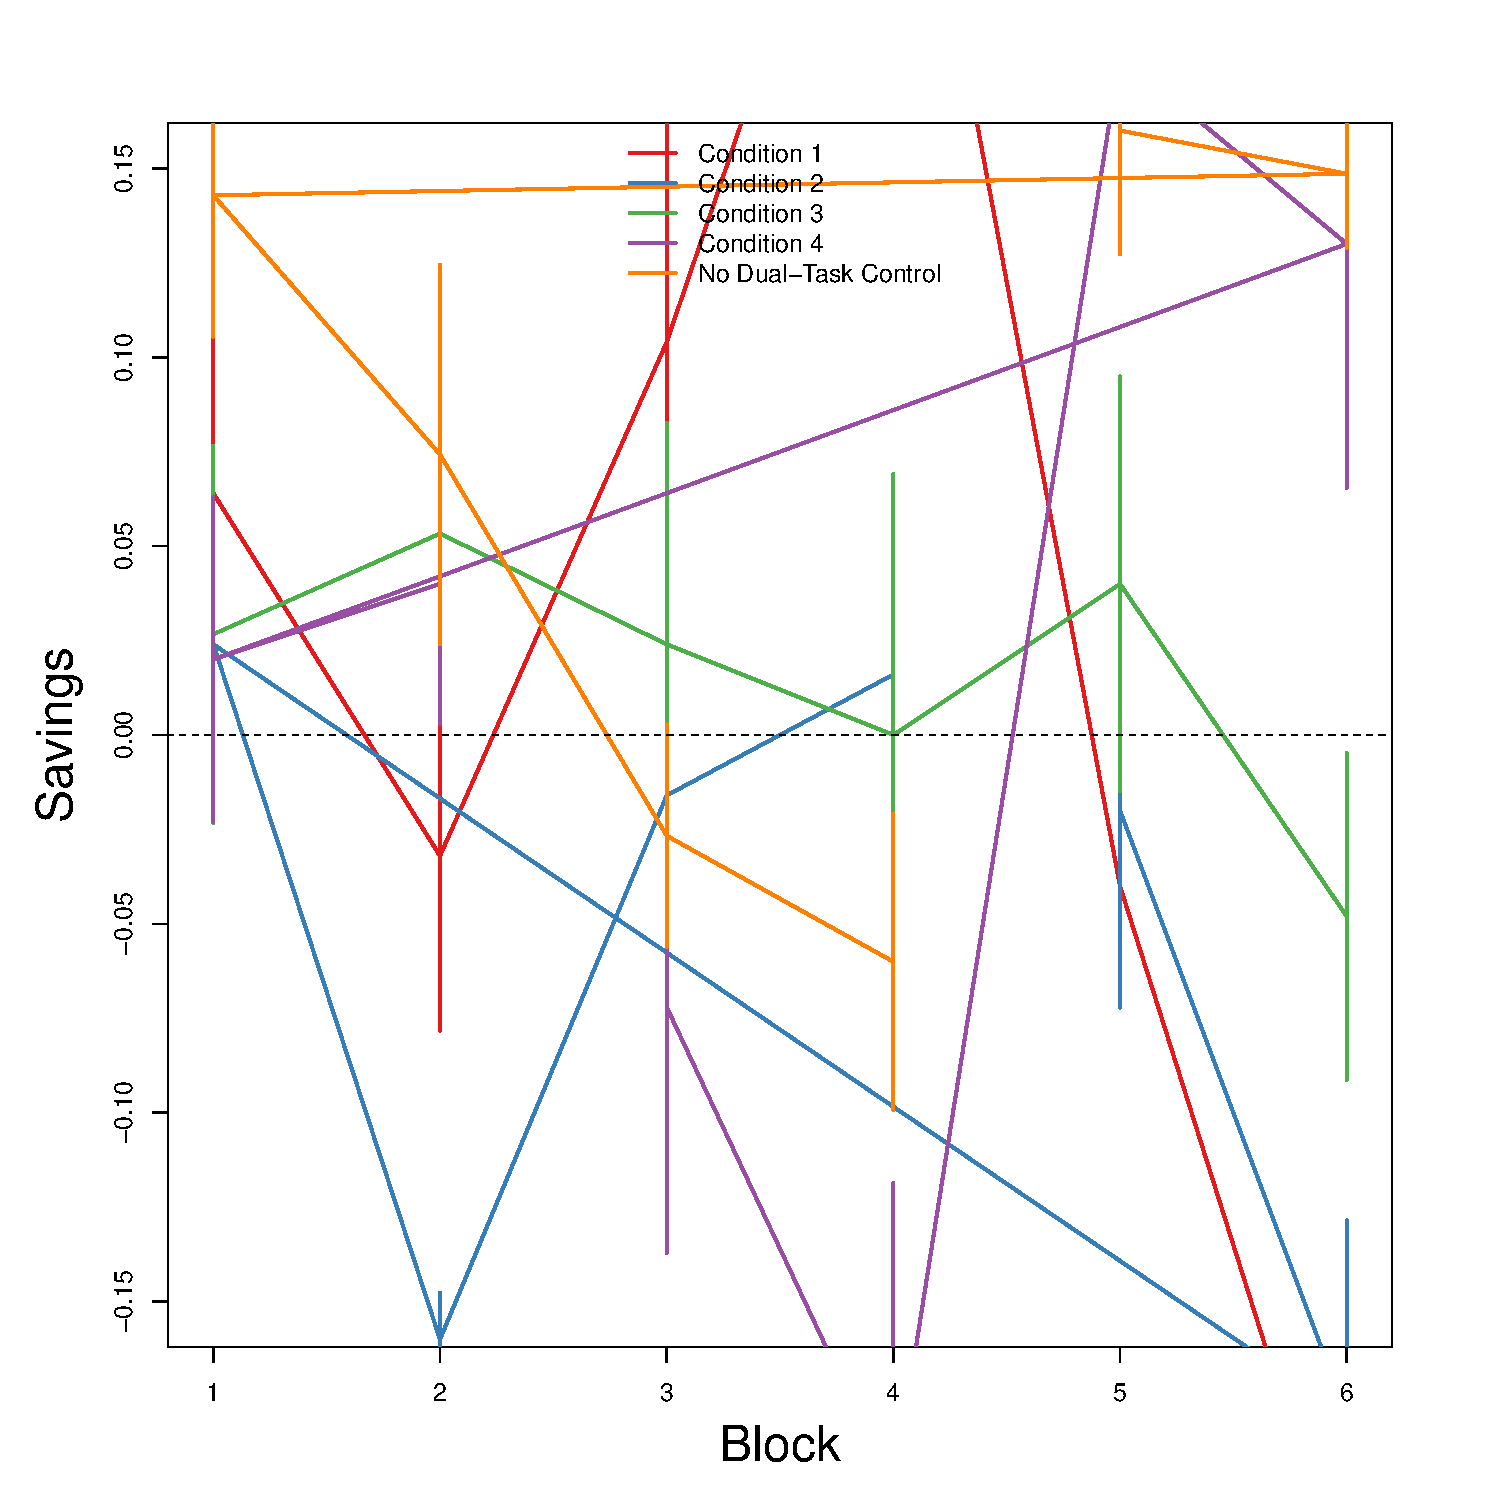
\includegraphics[width=1.0\textwidth]{../figures/fig_savings_per_block.pdf}
  \caption{ Savings (reacquisition - acquisition) per 25 trial block. Error bars
    are SEM. }
  \label{fig:savings_per_block}
\end{figure}

If the computation of feedback contingency depends on declarative systems, then
we expect the dual-task conditions to exhibit less savings than the no dual-task
control -- that is, we expect reacquisition of the original categories to be
slower under dual-task conditions. This is apparent via visual inspection of
Figure \ref{fig:learning_curves} (e.g., the red lines are always below the blue
line), and also of Figure \ref{fig:savings}, which shows the savings observed
for every participant in every condition as a box plot with individual
participant data points superimposed. As a comparison, Figure \ref{fig:savings}
also shows the results from the random-feedback intervention condition of
Crossley et al. (2013), which was similar in design to our no dual-task control
condition (although the Crossley et al. condition included fewer intervention
trials).

Figure \ref{fig:savings_per_block} shows the savings during each 25-trial block,
where savings is defined as reacquisition accuracy minus acquisition accuracy on
the block in the same ordinal order (e.g., first reacquisition block accuracy
minus first acquisition block accuracy, etc.). Several features of these data
are worth noting. First, savings in the no dual-task control condition is
uniformly greater than in any other condition. Second, there is little
difference in savings in any dual-task condition. Third, in every condition, the
curves are decreasing, and fourth, in every case, savings become negative,
indicating that asymptotic accuracy during reacquisition was lower than during
acquisition in every condition.

These observations are supported via the results of a 5 condition $\times$ 6
block ANOVA. There was a significant effect of Condition [$F(1,974) = 5.77, p <
0.05, \Omega^2 = 0.01$], indicating less savings in the dual-task conditions
relative to the no dual-task condition. There was a significant effect of Block
[$F(1,974) = 22.55, p < 0.001, \Omega^2 = 0.02$], indicating that savings in all
conditions was most prominent during early blocks and gradually decreased (see
Figure \ref{fig:savings_per_block}). The Condition $\times$ Block interaction
was n.s. [$F(1,974) = 0.001$, $p = 0.97, \Omega^2 = 0.00$].
    
The directional interpretation of these omnibus tests is supported by several
planned comparisons. First, Condition 2 savings were significantly less than in
the no dual-task control condition [$t(63) = 2.09, p = 0.04, d = 0.55$], whereas
savings in the other dual-task conditions were all marginally less than in the
control condition [condition 1 < control: $t(46) = -1.24, p = 0.22, d = 0.22$;
condition 3 < control: $t(57) = -1.63, p = 0.11, d = 0.35$; condition 4 <
control: $t(61) = -1.67, p = 0.10, d = 0.36$]. Second, there were no significant
differences in savings between any dual-task conditions \footnote{Note that the
following p-values should all be corrected for multiple comparisons. However,
any such correction would only increase each p value, and therefore would not
change our nonsignificance conclusions.} [condition 1 > condition 2: $t(53) =
0.37, p = 0.71, d = 0.02$; condition 1 > condition 3: $t(56) = 0.12, p = 0.90, d
= 0.00$; condition 1 > condition 4: $t(53) = 0.08, p = 0.94, d = 0.00$;
condition 2 > condition 3: $t(63) = -0.29, p = 0.78, d = 0.01$; condition 2 >
condition 4: $t(65) = -0.36, p = 0.72$, $d = 0.02$; condition 3 > condition 4:
$t(62) = -0.06, p = 0.96, d = 0.00$].

\subsubsection*{Participant-Level Savings} 
\begin{figure}[t]
\centering 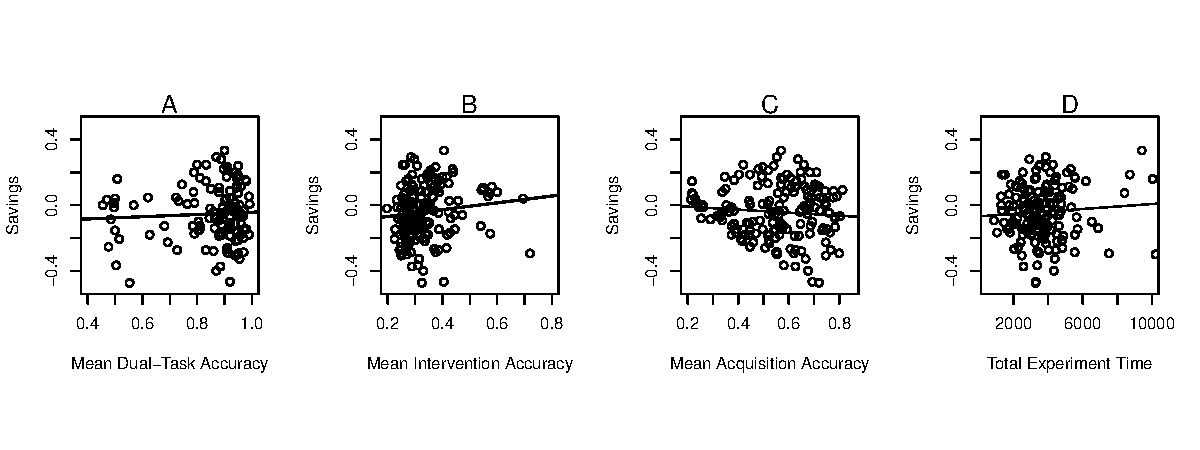
\includegraphics[width=1.0\textwidth]{../figures/fig_save_mixed_2.pdf}
  \caption{ 
    Regression analyses to examine possible predictor variables for savings.
    A: Mean dual-task accuracy.
    B: Mean Intervention accuracy. 
    C: Mean acquisition accuracy.
    D: Total experiment time.
  }
  \label{fig:savings_mixed}
\end{figure}

Figure \ref{fig:savings} shows large individual differences -- with many
participants in all conditions expressing both positive and negative savings.
This section describes the results of an exploratory analysis that examines what
factors might predict savings in individual participants. In particular, we
performed a multiple regression with three predictors: (1) mean dual-task
accuracy, (2) mean intervention accuracy, and (3) mean acquisition accuracy.
Dual-task performance might reflect the degree to which the computation of
feedback contingency is impaired, and thereby predict savings. Mean intervention
accuracy may reflect the degree to which procedural knowledge is being
expressed, and therefore is vulnerable to modification. Mean acquisition
accuracy may predict savings in that the stronger initial learning, the more
robust to intervention it may be, and the more likely it should be manifest as
savings in relearning.

Figure \ref{fig:savings_mixed} plots savings against each of these predictor
variables. Note that data was pooled across the four dual-task conditions for
this analysis. The regression revealed a significant negative coefficient for
mean acquisition performance ($\beta=-0.23, t(125)=-2.17, p<.05$), showing that
the better a participant did during acquisition, the less savings they were
likely to express. The coefficient for mean intervention performance was
positive and nearly significant ($\beta=.30, t(125)=1.79, p=.07$), showing that
there was a trend for higher intervention accuracy to predict better savings.
The coefficient for mean dual-task performance was not significantly different
from zero ($\beta=.09, t(125)=.87, p=.39$). The overall model, however, was not
a very good predictor of savings, explaining a nearly significant proportion of
variance in savings ($R^2=.05, F(3,125)=2.29, p=.08$).

Our results show less savings in dual-task conditions than in the the no
dual-task control, and also show no significant differences in savings between
dual-task conditions. It therefore seems possible that our results may simply
reflect that categorization with a dual-task is more tiring than categorization
without a dual task. However, this possibility does not survive a closer
inspection at our data. First, if participant fatigue is the driving factor,
then there should be differences between the dual-task conditions, which we did
not observe. Second, we performed a linear regression with overall experiment
time as the predictor variable. The idea here is that the longer the experiment
took, the more fatigue a participant should be vulnerable to, and the less
savings they should express. Note that we performed this regression on the
pooled data from all five experimental conditions. The coefficient for total
experiment time was not significantly different from zero ($\beta=7.5 \times
10^-6, t(161)=.93, p=.35$), and did not predict a significant proportion of
variance in savings ($R^2=.005, F(1,161)=.87, p=.35$).

% Matt: I'm a little worried that we're setting ourselves up here for criticism.
% Couldn't a reviewer just extend this argument and say something like the
% following: ``Categorization with a dual task is more tiring than categorization
% without a dual task. Maybe the only thing the dual task did was fatigue subjects
% and that the effect of this was to essentially just shift the savings vs blocks
% plots to the right (e.g., note that if you shift the dual task plots 2 blocks to
% the right they largely overlap the no dual-task control curve).

%MATT: I really like the idea but this section needs work. First, please add labels to each plot in the figures. I assume that the four plots in each figure refer to the four dual-task conditions, but this isn't obvious. Second, 3 of the 4 slopes in Fig. 9 are positive. It's easy to test significance here (either a t test on slope or test that r^2 = 0). Are any of these significant? Third, it seems to me that you really should just do a single multiple regression with three predictors.

% \subsection*{Decision-Bound Modeling} 
% \begin{figure}[t]
%   \centering 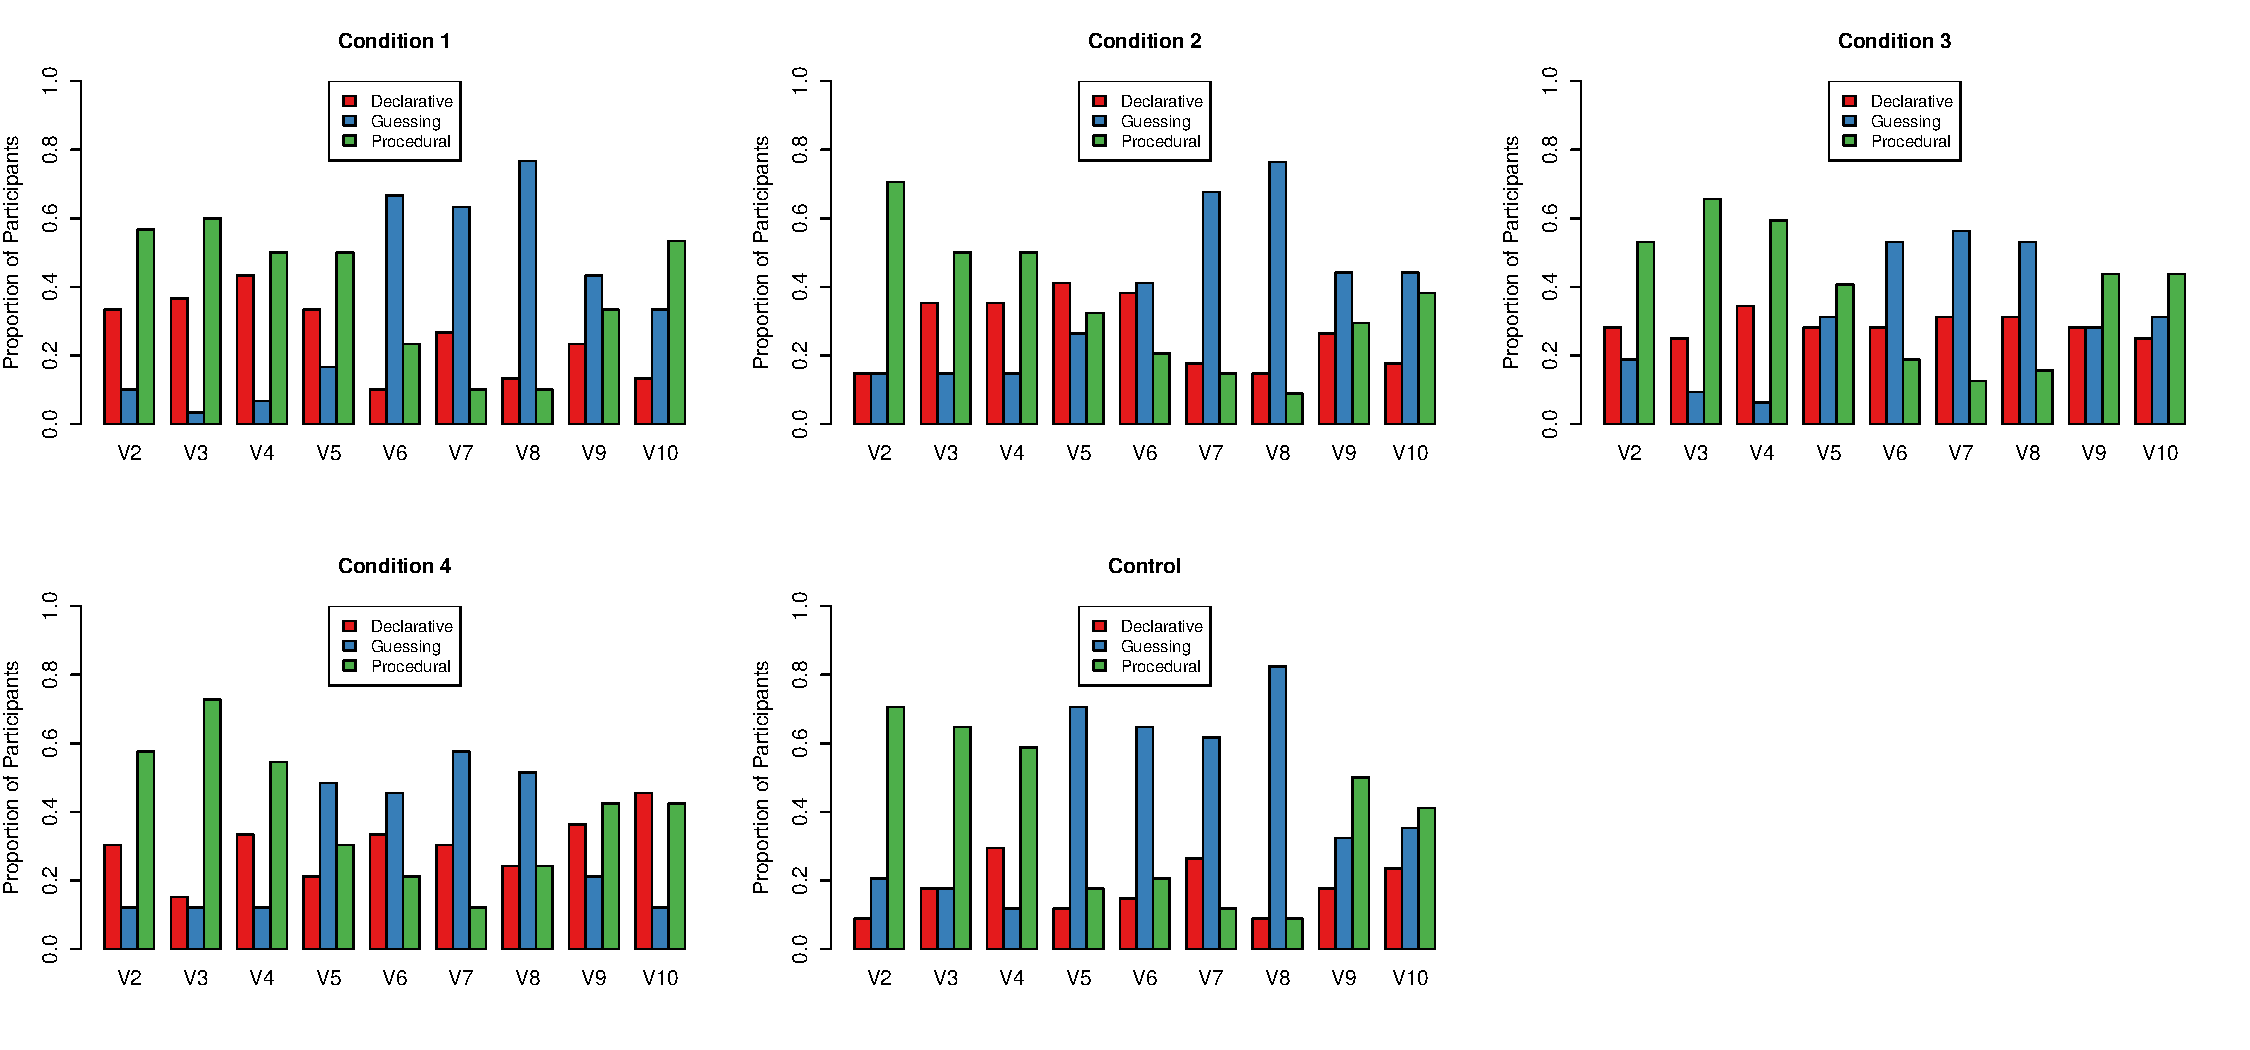
\includegraphics[width=1.0\textwidth]{../figures/fig_model_fits.pdf}
%   \caption{
%     Proportion of participants best fit by a decision-bound model assuming a
%     procedural, declarative, or guessing strategy. The key feature of this
%     figure is that participants in the no dual-task control condition changed
%     their response strategy more during the intervention more quickly than
%     participants in all dual-task conditions. 
%     \textbf{A:} Condition 1 (dual-task applied on trial 251 through trial 350).
%     \textbf{B:} Condition 2 (dual-task applied on trial 251 through trial 450). 
%     \textbf{C:} Condition 3 (dual-task applied on trial 251 through trial 550). 
%     \textbf{D:} Condition 4 (dual-task applied on trial 351 through trial 650). 
%     \textbf{E:} Condition 5 (no dual-task control). 
%   }
%   \label{fig:exp_fits}
% \end{figure}
